\documentclass[12pt,a4paper]{article}
\usepackage[utf8]{inputenc}
\usepackage[finnish]{babel}
\usepackage{setspace}
%\usepackage{parskip}
%\usepackage{amssymb}
%\usepackage{amsmath}
\usepackage{graphicx}
\usepackage{subcaption}
\usepackage{fancyhdr}
\usepackage[top=1in, bottom=1in, left=1in, right=1in]{geometry}
\usepackage{float}
\usepackage[section]{placeins}
\usepackage[nottoc,notlot,notlof]{tocbibind}

\usepackage{titlesec}
\titleclass{\section}{top}
\newcommand\sectionbreak{\clearpage}
\titleformat*{\section}{\Huge\bfseries}
\titleformat*{\subsection}{\Large\bfseries}
\titleformat*{\subsubsection}{\large\bfseries}

%\usepackage[numbered,autolinebreaks,useliterate]{mcode} % jos tahdot laittaa matlabkoodia näkyville niin kannattaa käyttää tätä

% hyödyllisiä paketteja:
\usepackage{siunitx}\sisetup{per=frac} % SI-yksiköitä.
%\usepackage{supertabular} % jos tarttee isoja taulukoita
%\usepackage{fullpage} % pienemmät marginaalit jos haluaa

\usepackage{hyperref} % lisääthän omat pakettisi ENNEN hyperref'iä
\hypersetup{pdfborder={0 0 0}}
\onehalfspacing
\cfoot{}
%\rhead{\thepage}
% asettaa nyk. kappaleen nimen vasempaan ylänurkkaan, saa poistaa jos haluaa
%\lhead{\leftmark}

%%%%% kaikki ennen tätä liittyy käytettäviin paketteihin tai dokumentin muotoiluun. siihen ei tarvinne aluksi koskea. %%%%%

\begin{document}
%\newgeometry{top=1in, bottom=1.5in, left=1.5in, right=1.5in}
%%\begin{abstract}
%%\setlength{\parindent}{0pt}
%%\parskip=1em \advance\parskip by 0pt plus 2pt
%%\onehalfspacing
%
%%%%%% Tiivistelmäteksti %%%%%
%\noindent
%Tyrkkää tänne tiivis tiivistelmä tuloksista.
%
%\LaTeX saattaa tuntua aluksi hankalalta. Valmiin pohjan käyttäminen on kuitenkin helppo tapa päästä jyvälle, niin allekirjoittanutkin aikoinaan oppi. Netistä löytyy myös paljon materiaalia, esim wikibooksista (\url{http://en.wikibooks.org/wiki/LaTeX}). Myös suomenkielistä materiaalia on: \url{http://www.cs.tut.fi/lintula/manual/TeX/TeXdoc/latex/general/lyhyt/lyhyt2e.pdf}. Ette te kuitenkaan tuota jaksa lukea, en minäkään jaksanut, mutta tiedättepähän että on mistä etsiä jos on ongelmia. Suosittelen myös googlea: kaltaisiani hönöjä on internet täynnä joten esimerkiksi stack\-ex\-changessa % jos ihmettelet tuota \- niin se on tavutusvihje. Aina latexin kääntäjä ei osaa tavuttaa sanoja oikein, jolloin sille voi kertoa parhaan paikan katkaista sana. Jos ihmettelet tätä prosenttimerkillä alkavaa osaa, tämä on kommentti. Niihin voi kirjoittaa kaikenlaista sellaista, minkä ei tahdo tulevan näkyviin lopulliseen dokumenttiin.
%joku on jo kysynyt lähes jokaista minulle eteen tullutta ongelmaa. Näpyttäkää siis ongelmanne googleen avainsanan "latex" kanssa.
%
%Jos opettelu tuntuu vaikealta, kannattaa muistaa, että fyysikolle se on edessä ennemmin tai myöhemmin joka tapauksessa. Tähtitieteilijälle jo ennemmin: tähtitieteen käytännön menetelmien lopputyö pitää laatia latexilla.
%
%Tämä selkkaripohja on tehty Helsingin Matematiikkalukiossa käytetyn tutkielmapohjan päälle, kiitokset siitä Tuomas Tynkkyselle.
%
%\-Rakkaudella kaikille fukseille ja fuksinmielisille $\heartsuit$ \\
%Anni Järvenpää
%\end{abstract}
%\restoregeometry

% Sisällysluettelo
\newpage
\thispagestyle{empty}
\tableofcontents
\newpage
\setcounter{page}{1}
\parskip=1em \advance\parskip by 0pt plus 2pt
\pagestyle{fancy}


%%%%%%%%%%%%%%% Oleellinen sisältö alkaa%%%%%%%%%%%%%%%
\section{Johdanto}



\cite{rj, yt, enzo}

%Teoreettista teoriaa. Täällä tarvitaan myös yhtälöitä, yhtälö \ref{esimerkkiyhtalo} on yksi sellainen.
%
%\begin{equation}\label{esimerkkiyhtalo}
%	c=\sqrt{a^2+b^2}
%\end{equation}

%\begin{align} % &-merkki kertoo mitkä kohdat laitetaan päällekkäin
%s_{1} =& d \cos \alpha = d \cos (90 \,^{\circ} - \varphi) = d \sin \varphi \label{align1} \\
%s_{2} =& d \cos \beta = d \cos (90 \,^{\circ} - \theta) = d \sin \theta \label{align2},
%\end{align}
%\begin{align}
%\lambda&=\frac s n \nonumber \\
%&= \frac{s_1-s_2}{n} \nonumber \\
%&= \frac{d}{n} ( \sin \varphi - \sin \theta ) \label{sievennystulos}
%\end{align}

%\begin{equation*}
%	\sin{x} \approx x \text{ kun x on pieni}
%\end{equation*}


\section{Enzo}
Enzo on adaptiivista verkontihennystä (\textit{Adaptive Mesh Refinement}, AMR) hyödyntävä simulaatiokoodi, %TODO mieti: adaptiivinen verkontihennys, jotain muuta? simulaatiokoodi?
joka mahdollistaa ympäristöä suuremman aika- ja paikkaresoluution käyttämisen simulaation kiinnostavilla alueilla. Tämä on tärkeää, sillä usein melko pienellä alueella tarvitaan suurta resoluutiota, mutta koko simulaation ajaminen näin suurella tarkkuudella veisi kohtuuttoman paljon aikaa. Siksi AMR-simulaatioissa simulaation solun kokoa voidaan muuttaa  % eri kokoiset lootikot

Esimerkiksi kuvassa \ref{fig:enzogrid} nähdään, kuinka tiheämmillä alueilla käytetään pienempiä 

\begin{figure}
   \centering
   \begin{subfigure}[b]{0.45\textwidth}
       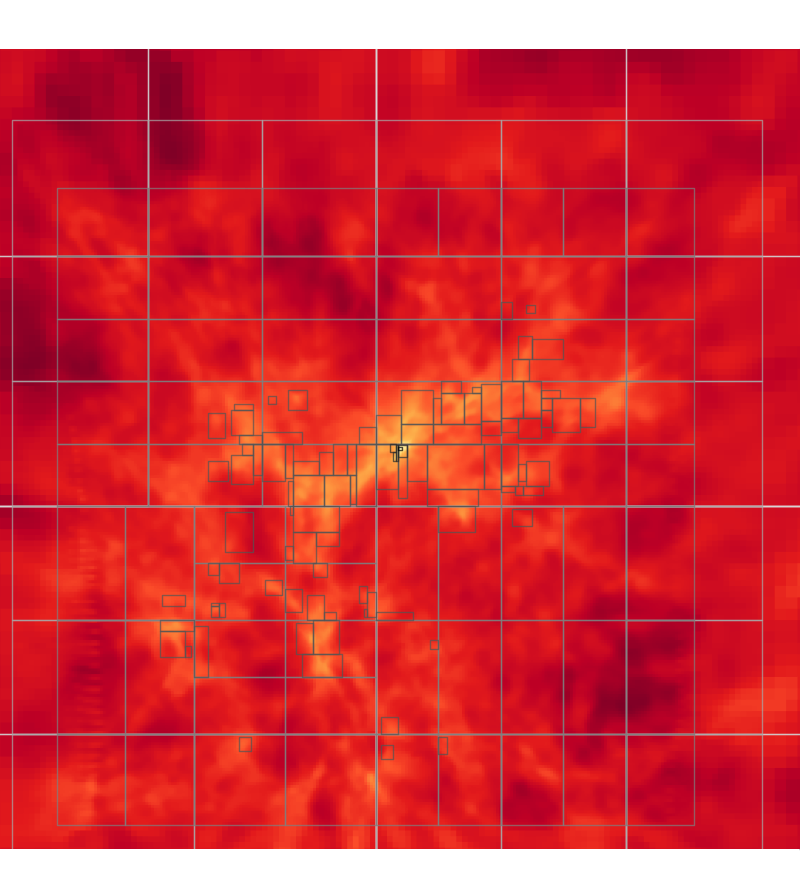
\includegraphics[height=7.5cm]{../kuvat/amr-grid.png}
       %\caption{}
       %\label{fig:gull}
   \end{subfigure}
   \begin{subfigure}[b]{0.45\textwidth}
       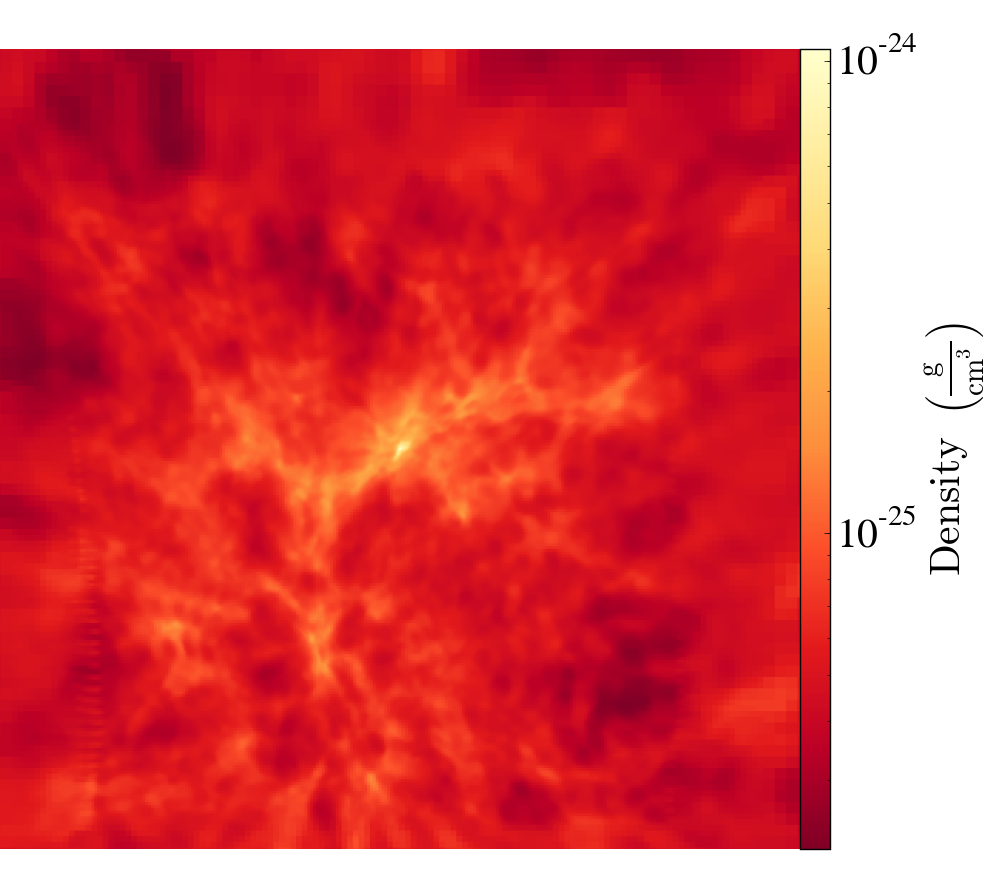
\includegraphics[height=7.5cm]{../kuvat/amr-nogrid.png}
       %\caption{A tiger}
       %\label{fig:tiger}
   \end{subfigure}
   \caption{Halkileikkaus $100$ pc$^2$ alueesta erään Enzo-simulaation alkutilanteesta solujen raajat näkyvillä (vasen kuva) sekä ilman niitä (oikea kuva). Kiinnostavammilla alueilla solut ovat pienempiä. Resoluution heikentyminen suuremmissa soluissa on selvästi nähtävissä.}\label{fig:enzogrid} %TODO mieti: miten näkyviin se, että kyseessä on Johnin simulaatio? Kerro mitä kuvassa on

\end{figure}

\section{\texttt{yt}}
waaaiiiitiiii

%\begin{figure}
%\centering
%\includegraphics[width=\textwidth]{yllatyskipsu.jpg} %lveydeksi voi antaa myös vaikkapa 5cm tai muun konkreettisen mitan tai vaihtoehtoisesti asettaa leveydeksi vaikapa 80% tekstin leveydestä parametrilla 0.8\textwidth. Kuvan korjeuden voi asettaa esimerkiksi height=6cm.
%\caption{Kuvatekstissä voisin vaikkapa kertoa, että oikeasti kissa vain haukottelee.}
%\label{kissakuva}
%\end{figure}

\section{Oma työ}
joo kyl mäki tein jotain


\section{Tulokset}
tulostan tähän tuloksia


\section{Loppupäätelmät}
paska työ mutta tulipahan tehtyä


%%%%% Sisältö loppuu, lähdeluettelo %%%%%
\bibliographystyle{plain}
\bibliography{lahteet}

\appendix
\newpage
\section{Liittyvä liite.} \label{koodi}
Liian laaja leipätekstiin.
\end{document}
